\section{Trasformata di Burrows--Wheeler posizionale}
\label{secpbwt}
Presentata nel 2014 da Richard Durbin \cite{pbwt}, la \textbf{Positional
  Burrows--Wheeler Transform} ($\PBWT$), traducibile con
\textit{trasformata di Burrows--Wheeler posizionale}, è una struttura dati
efficiente
per la memorizzazione e l'interrogazione di pannelli di aplotipi.\\
La costruzione di tali pannelli avviene tramite il riconoscimento delle
varianti di un singolo nucleotide tra le sequenze genomiche di diversi
individui, ovvero dei cosiddetti Single-Nucleotide Polymorphism
(SNP). Ogni variante, identificata per un certo nucleotide in una
posizione specifica, viene 
detto allele. La combinazione di tutte le varianti alleliche,
ereditate, a meno di mutazioni, da ogni genitore, forma l'\textbf{aplotipo} di
un certo individuo. Come visibile in figura \ref{fig:haplo} \cite{haplo}, la 
costruzione parte da diversi sequenziamenti (nell'immagine relativi a diversi
cromosomi ma il
procedimento è uguale partendo da diversi individui) grazie a cui si
identificano le 
varianti alleliche. Da queste ultime si costruiscono gli aplotipi, utilizzati
per estrarre i cosiddetti tag SNP, ovvero le possibili alternative per
una certa variante allelica. Questi ultimi, normalmente rappresentati per
l'uomo da due caratteri vista la sua natura diploide, formano,
l'alfabeto del pannello. 
L’informazione combinata di tutti gli aplotipi in un individuo è detta
\textbf{genotipo}.
\begin{figure}
  \centering
  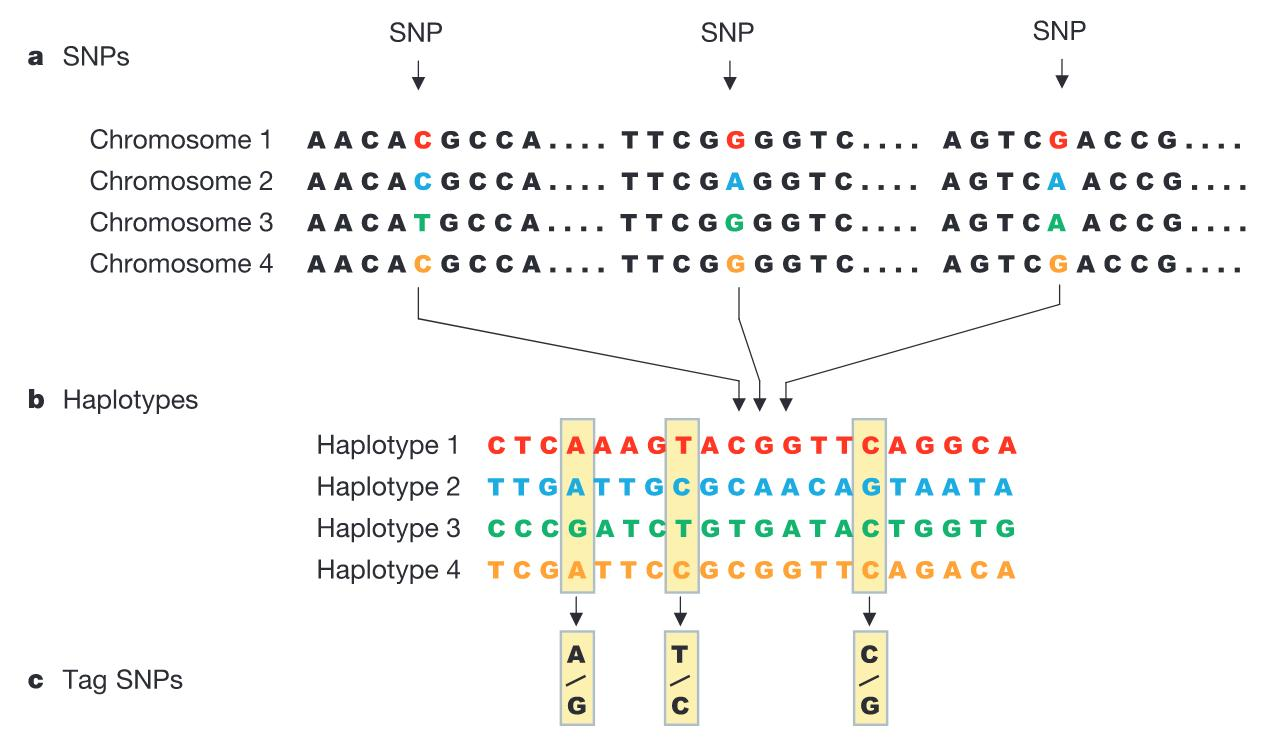
\includegraphics[scale = 0.25]{img/haplo.jpg}
  \caption{Schema di ottenimento del pannello di aplotipi.}
  \label{fig:haplo}
\end{figure}
Formalmente, si considera un pannello $X$ di $M$ aplotipi $x_i$, con
$i=0,\ldots, M-1$, con $N$ siti, indicizzati tramite $k=0,\ldots, N-1$, tale per
cui tutti i siti sono considerati biallelici. 
Da un punto di vista computazionale, quest'ultima
assunzione comporta che il pannello $X$ è costruito sull'alfabeto ordinato
$\Sigma =\{0,1\}$, con $0\prec 1$, avendo la sostituzione dei tag SNPs,
per un certo sito, con tale alfabeto. Ne segue che:
\begin{equation}
  \label{eq:pbwtdip}
  x_i[k]=\{0,1\}
\end{equation}
Prima di proseguire con la trattazione, è bene specificare alcuni
formalismi utilizzati:
\begin{itemize}
  \item si denota con $x_i[k_1,k_2)$ la
  sottostringa di $x_i$ che inizia alla colonna $k_1$ e termina alla
  colonna $k_2-1$, per una qualsiasi riga $x_i\in X$
  \item date due righe $x_i$ e $x_j$, si ha un match tra le due
  righe, iniziante
  alla colonna $k_1$ e terminante alla colonna $k_2-1$, sse:
  \begin{equation}
    \label{eq:pbwtmatch}
    x_i[k_1,k_2)=x_j[k_1,k_2)
  \end{equation}
  \item un match tra due righe $x_i$ e $x_j$, come definito al punto precedente,
  è definito localmente massimale sse non si ha alcuna estensione a
  destra o sinistra che comporti un ulteriore match:
  \begin{equation}
    \label{eq:pbwtmem}
    (k_1=0\lor x_i[k_1-1]\neq x_j[k_1-1])\land (k_2=N\lor x_i[k_2]\neq x_j[k_2])
  \end{equation}
  \item comparando una sequenza (ovvero un aplotipo esterno) $z$ a un pannello
  di aplotipi $X$, si ha che un match
  localmente massimale è un
  set-maximal exact match ($\SMEM$) di $z$ contro $x_i\in X$, iniziante 
  alla colonna $k_1$ e terminante alla colonna $k_2-1$,
  sse non si ha alcun altro match localmente
  massimale di $z$ con un 
  altro $x_j$ che include ed estende l'intervallo $[k_1,k_2)$. La sequenza $z$
  può avere uno $\SMEM$, tra $k_1$ e $k_2-1$, con più di un aplotipo del
  pannello. Per praticità, si è introdotta la definizione di $\SMEM$ usando un
  aplotipo esterno, ma tale definizione può essere riferita anche a due righe
  interne al pannello $X$
\end{itemize}
Si noti che il match tra due sequenze nella $\PBWT$ è tale sse entrambi iniziano
e terminano nella stessa colonna. Questo vincolo,
da cui deriva il termine ``posizionale'' e che impedisce l'uso degli
algoritmi tradizionali visti con la $\BWT$, è dato dal fatto che una
colonna rappresenta un preciso sito di una variante genica. \\
La costruzione di questa struttura dati si basa, a ogni colonna $k$, sul
riordinamento lessicografico delle sequenze di aplotipi, nel dettaglio
sull'ordinamento 
inverso dei prefissi terminanti in colonna $k-1$. I valori presenti in colonna
$k$, dopo il riordinamento, sono quelli che andranno a popolare
la cosiddetta matrice $\PBWT$, che rappresenta la vera e propria
trasformata. Si noti che avere le sequenze 
ordinate in base ai prefissi inversi alla $k$-esima colonna permette di
identificare i match con maggior facilità in quanto aplotipi
con suffisso comune (o prefisso comune inverso) saranno ``virtualmente'' in
posizioni 
consecutive a ogni riordinamento della trasformata.\\
Il calcolo di tutti i riordinamenti non presenta difficoltà dal punto di
vista computazionale. Infatti, conoscendo l'ordinamento in colonna $k$, si può
derivare facilmente quello in colonna $k+1$, studiando solo i valori
riordinati alla colonna precedente. Si ha infatti un ordinamento stabile ad ogni
colonna. 
\begin{definizione}
  Dato un pannello $X$ e un indice di colonna
  $k$, si definisce il \textbf{prefix array} $a_k$ come una permutazione degli
  indici $\{0,\ldots, M-1\}$ tale per cui $a_k[i]=j$ sse $x_j$ è l'$i$-esimo
  aplotipo di 
  $X$ nell'ordinamento inverso dei prefissi ottenuto alla colonna $k$.
  % Quindi,
  % $a_k[i]=m$, con $m<M$, altro non è che l'indice della sequenza $x_m$ del
  % pannello $X$ da cui deriva il prefisso $i$-esimo nell'ordine inverso
  % in colonna $k$.
\end{definizione}
Data questa definizione, si ha che la matrice $\PBWT$ si ottiene
direttamente usando, per ogni colonna, gli indici del prefix
  array e prendendo i valori del pannello $X$ secondo l'ordine espresso da
esso.\\ 
Per comodità di rappresentazione, definiamo l'$i$-esima sequenza
nell'ordinamento inverso necessario a ottenere la colonna $k$ della matrice
$\PBWT$, come:
\begin{equation}
  \label{eq:pbwty}
  y_i^k=x_{a_k[i]}
\end{equation}
In termini di colonne, con la notazione
$y^k[k]$ si identifica l'intera colonna $k$ della matrice $\PBWT$ mentre
l'elemento $i$-esimo di tale colonna è indicizzato da $y_i^k[k]$.\\
L'ordinamento degli elementi per
$a_{k+1}$ si ottiene a partire 
dall'ordinamento in $a_k$, considerando i valori $y_i^k[k]$, $\forall
i\in\{0,M-1\}$, e la 
precedenza del valore 0 sul valore 1 per riordinare in modo stabile tali
valori.\\ 
Come anticipato, prefissi simili saranno consecutivi nei riordinamenti fino alla
colonna $k$-esima. Quindi, risulta utile tenere traccia della posizione iniziale
dei prefissi inversi comuni più lunghi tra prefissi adiacenti nei riordinamenti. 
\begin{definizione}
  Si definisce \textbf{divergence array} l'array $d_k$, tale che $d_k[i]$ è
  l'indice della colonna iniziale del match massimale a sinistra, terminante
  a destra in colonna
  $k-1$, tra 
  l'$i$-esimo aplotipo e il suo precedente nell'ordinamento ottenuto per la
  colonna $k$-esima. Formalmente, dato $i>0$, si definisce 
  $d_k[i]$ come il più piccolo $j$ tale che:
  \begin{equation}
    \label{eq:pbwtdiv}
    y_i^k[j,k)=y_{i-1}^k[j,k)
  \end{equation}
  Ne segue che:
  \begin{equation}
    \label{eq:pbwtdiv2}
    y_i^k[k-1]\neq y_{i-1}^k[k-1] \implies d_k[i]=k
  \end{equation}
  Per definizione, non avendo una riga precedente con cui effettuare il
  confronto, si ha che $d_k[0]=k$.
\end{definizione}
Si noti che, per le proprietà del divergence array, l'inizio di qualsiasi match
massimale, terminante 
in colonna $k$, tra qualsiasi $y_i^k$ e $y_j^k$, con $i<j$, è dato da:
\begin{equation}
  \label{eq:pbwtint}
  \max_{i<m\leq j}d_k[m]
\end{equation}
Al posto del divergence array si può usare anche una
variante ``posizionale'' del Longest Common Prefix array.
\begin{definizione}
  Si definisce Reverse Longest Common Prefix ($\,\RLCP$) l'array $l_k$
  che, anziché 
  memorizzare l'indice d'inizio del match massimale a sinistra da due aplotipi
  consecutivi nell'ordinamento ottenuto alla colonna $k$-esima, tiene traccia
  della lunghezza di tale match. Formalmente si ha che:
  \begin{equation}
    \label{eq:pbwtlcp}
    l_k[i]=k-d_k[i]
  \end{equation}
\end{definizione}
\noindent
Fatte queste premesse possiamo quindi fornire una definizione formale di
$\PBWT$.
\begin{definizione}
  Dato un pannello $X=\{x_0,x_1,\ldots,x_{M-1}\}$, di $M$ aplotipi con ciascuno
  $N$ siti, si definisce $\PBWT$ di $X$ una
  collezione di $N+1$ coppie di array $(a_k,d_k)$, con $0\leq k\leq N$.
\end{definizione}
La procedura per la costruzione di $a_{k+1}$ e $d_{k+1}$ a partire da $a_k$ e
$d_k$ è disponibile all'algoritmo \ref{algo:durbin1}. Si noti che
il costo della costruzione dei due insiemi di array è:
\begin{equation}
  \label{eq:pbwtadtime}
  \mathcal{O}(NM)
\end{equation}
Ai fini della trattazione dell'algoritmo di computo degli $\SMEM$ per
un aplotipo esterno,
ricordiamo un'ulteriore definizione, analoga
a quanto visto con il suffix array e la sua permutazione inversa. 
\begin{definizione}
  Si definisce $\alpha_k$ come l'inverso della permutazione data dal
  prefix array $a_k$, avendo che:
  \[\alpha_k[i]=j \iff a_k[j]=i\]
\end{definizione}
Grazie a queste prime definizioni, è possibile denotare alcune forti
correlazioni, esplicitate in tabella \ref{tab:pbwtbwt}, che sussistono tra 
$\BWT$ e $\PBWT$ (e le rispettive varianti run-length
encoded), fattori chiave nello sviluppo di
questa tesi.
\begin{table}
  \centering
  \caption{Tabella di confronto tra le strutture dati relative alla $\BWT$ e
    alla $\PBWT$.}
  \label{tab:pbwtbwt}
  \begin{tabular}{c|c}
    $\BWT$ & $\PBWT$\\
    \hline
    $\SA_T$ & $a_k$\\
    $\ISA_T$ & $\alpha_k$\\
    $\LCP_T$ & $d_k$ o $l_k$\\            
  \end{tabular}
  
\end{table}
\begin{algorithm}
  \small
  \begin{algorithmic}[1]
    \Function{BuildPrefixAndDivergenceArrays}{$k$, $M$, $a_k$, $d_k$}
    \State $u\gets 0$, $v\gets 0$
    \State $p\gets k+1$, $q\gets k+1$
    \State $a\gets []$, $b\gets []$, $d\gets []$, $e\gets []$
    \For {\textit{every} $i\in[0,M-1]$}
    \If {$d_k[i]>p$}
    \State $p\gets d_k[i]$
    \EndIf
    \If {$d_k[i]>q$}
    \State $q\gets d_k[i]$
    \EndIf
    \If {$y_i^k[k]=0$}
    \State $a[u]\gets a_k[i]$, $d[u]\gets p$
    \State $u\gets u+1$, $p\gets 0$
    \Else
    \State $b[v]\gets a_k[i]$, $e[v]\gets q$
    \State $v\gets v+1$, $q\gets 0$
    \EndIf
    \EndFor
    \State $a_{k+1}\gets concatenate(a,b)$
    \State $d_{k+1}\gets concatenate(d,e)$ 
    \EndFunction
  \end{algorithmic}
  \caption{Algoritmo di Durbin per la costruzione di $a_{k+1}$ e $d_{k+1}$ a
  partire da $a_{k}$ e $d_{k}$.}
  \label{algo:durbin1}
\end{algorithm}
\newpage
\begin{esempio}
  \label{es:pbwt1}
  Dato il seguente pannello $X$ si vuole calcolare $y^6$:
  \begin{table}[H]
    \centering
    \scriptsize
    \begin{tabular}{c|ccccccccccccccc}
      X & 00 & 01 & 02 & 03 & 04 & 05 & 06 & 07 & 08 & 09 & 10 & 11 & 12 & 13
      & 14 \\
      \hline
      00 & 1 & 0 & 0 & 1 & 0 & 0 & 0 & 0 & 0 & 0 & 0 & 1 & 1 & 0 & 1 \\
      01 & 1 & 0 & 0 & 1 & 1 & 0 & 0 & 1 & 0 & 0 & 0 & 0 & 0 & 1 & 1 \\
      02 & 1 & 0 & 0 & 1 & 1 & 0 & 0 & 1 & 0 & 0 & 0 & 1 & 0 & 0 & 1 \\
      03 & 1 & 0 & 0 & 1 & 1 & 0 & 0 & 1 & 0 & 0 & 0 & 1 & 0 & 0 & 1 \\
      04 & 0 & 1 & 0 & 1 & 0 & 1 & 0 & 0 & 0 & 0 & 0 & 1 & 0 & 0 & 1 \\
      05 & 0 & 1 & 0 & 1 & 0 & 1 & 0 & 0 & 0 & 0 & 0 & 1 & 0 & 0 & 1 \\
      06 & 0 & 1 & 0 & 1 & 0 & 1 & 0 & 0 & 0 & 0 & 0 & 1 & 0 & 0 & 1 \\
      07 & 0 & 1 & 0 & 1 & 0 & 1 & 0 & 0 & 0 & 0 & 0 & 0 & 1 & 0 & 1 \\
      08 & 0 & 1 & 0 & 0 & 1 & 0 & 0 & 0 & 0 & 1 & 1 & 1 & 0 & 0 & 1 \\
      09 & 0 & 1 & 0 & 1 & 0 & 0 & 0 & 0 & 1 & 0 & 0 & 0 & 0 & 1 & 1 \\
      10 & 0 & 1 & 0 & 1 & 0 & 0 & 0 & 0 & 1 & 0 & 0 & 0 & 0 & 1 & 1 \\
      11 & 0 & 1 & 0 & 0 & 1 & 0 & 0 & 0 & 0 & 0 & 1 & 1 & 0 & 0 & 0 \\
      12 & 0 & 1 & 0 & 0 & 1 & 0 & 0 & 0 & 1 & 0 & 1 & 1 & 0 & 0 & 1 \\
      13 & 0 & 1 & 0 & 0 & 1 & 0 & 0 & 0 & 1 & 0 & 1 & 1 & 0 & 0 & 1 \\
      14 & 0 & 1 & 0 & 0 & 0 & 0 & 0 & 0 & 1 & 0 & 0 & 0 & 1 & 0 & 1 \\
      15 & 0 & 1 & 0 & 0 & 0 & 0 & 0 & 0 & 1 & 0 & 0 & 0 & 1 & 0 & 1 \\
      16 & 0 & 1 & 0 & 1 & 0 & 0 & 0 & 0 & 0 & 0 & 0 & 1 & 1 & 0 & 1 \\
      17 & 1 & 1 & 0 & 0 & 0 & 1 & 0 & 0 & 0 & 0 & 0 & 1 & 1 & 0 & 1 \\
      18 & 0 & 1 & 1 & 0 & 1 & 0 & 0 & 0 & 0 & 0 & 0 & 1 & 0 & 0 & 1 \\
      19 & 0 & 1 & 1 & 0 & 1 & 0 & 1 & 0 & 0 & 0 & 0 & 0 & 1 & 0 & 1 
    \end{tabular}
  \end{table}
  Si inizia riordinando il pannello con l'ordine inverso alla
  quinta colonna, avendo che $y^6$ è la sesta colonna del pannello
  così riordinato. Ne segue che, secondo il riordinamento mostrato nel seguente
  pannello, $a_6$ è la 
  colonna degli indici, già riordinati, mentre $d_6$ è specificato
  tramite le righe in verde:   
  \begin{figure}[H]
    \centering
    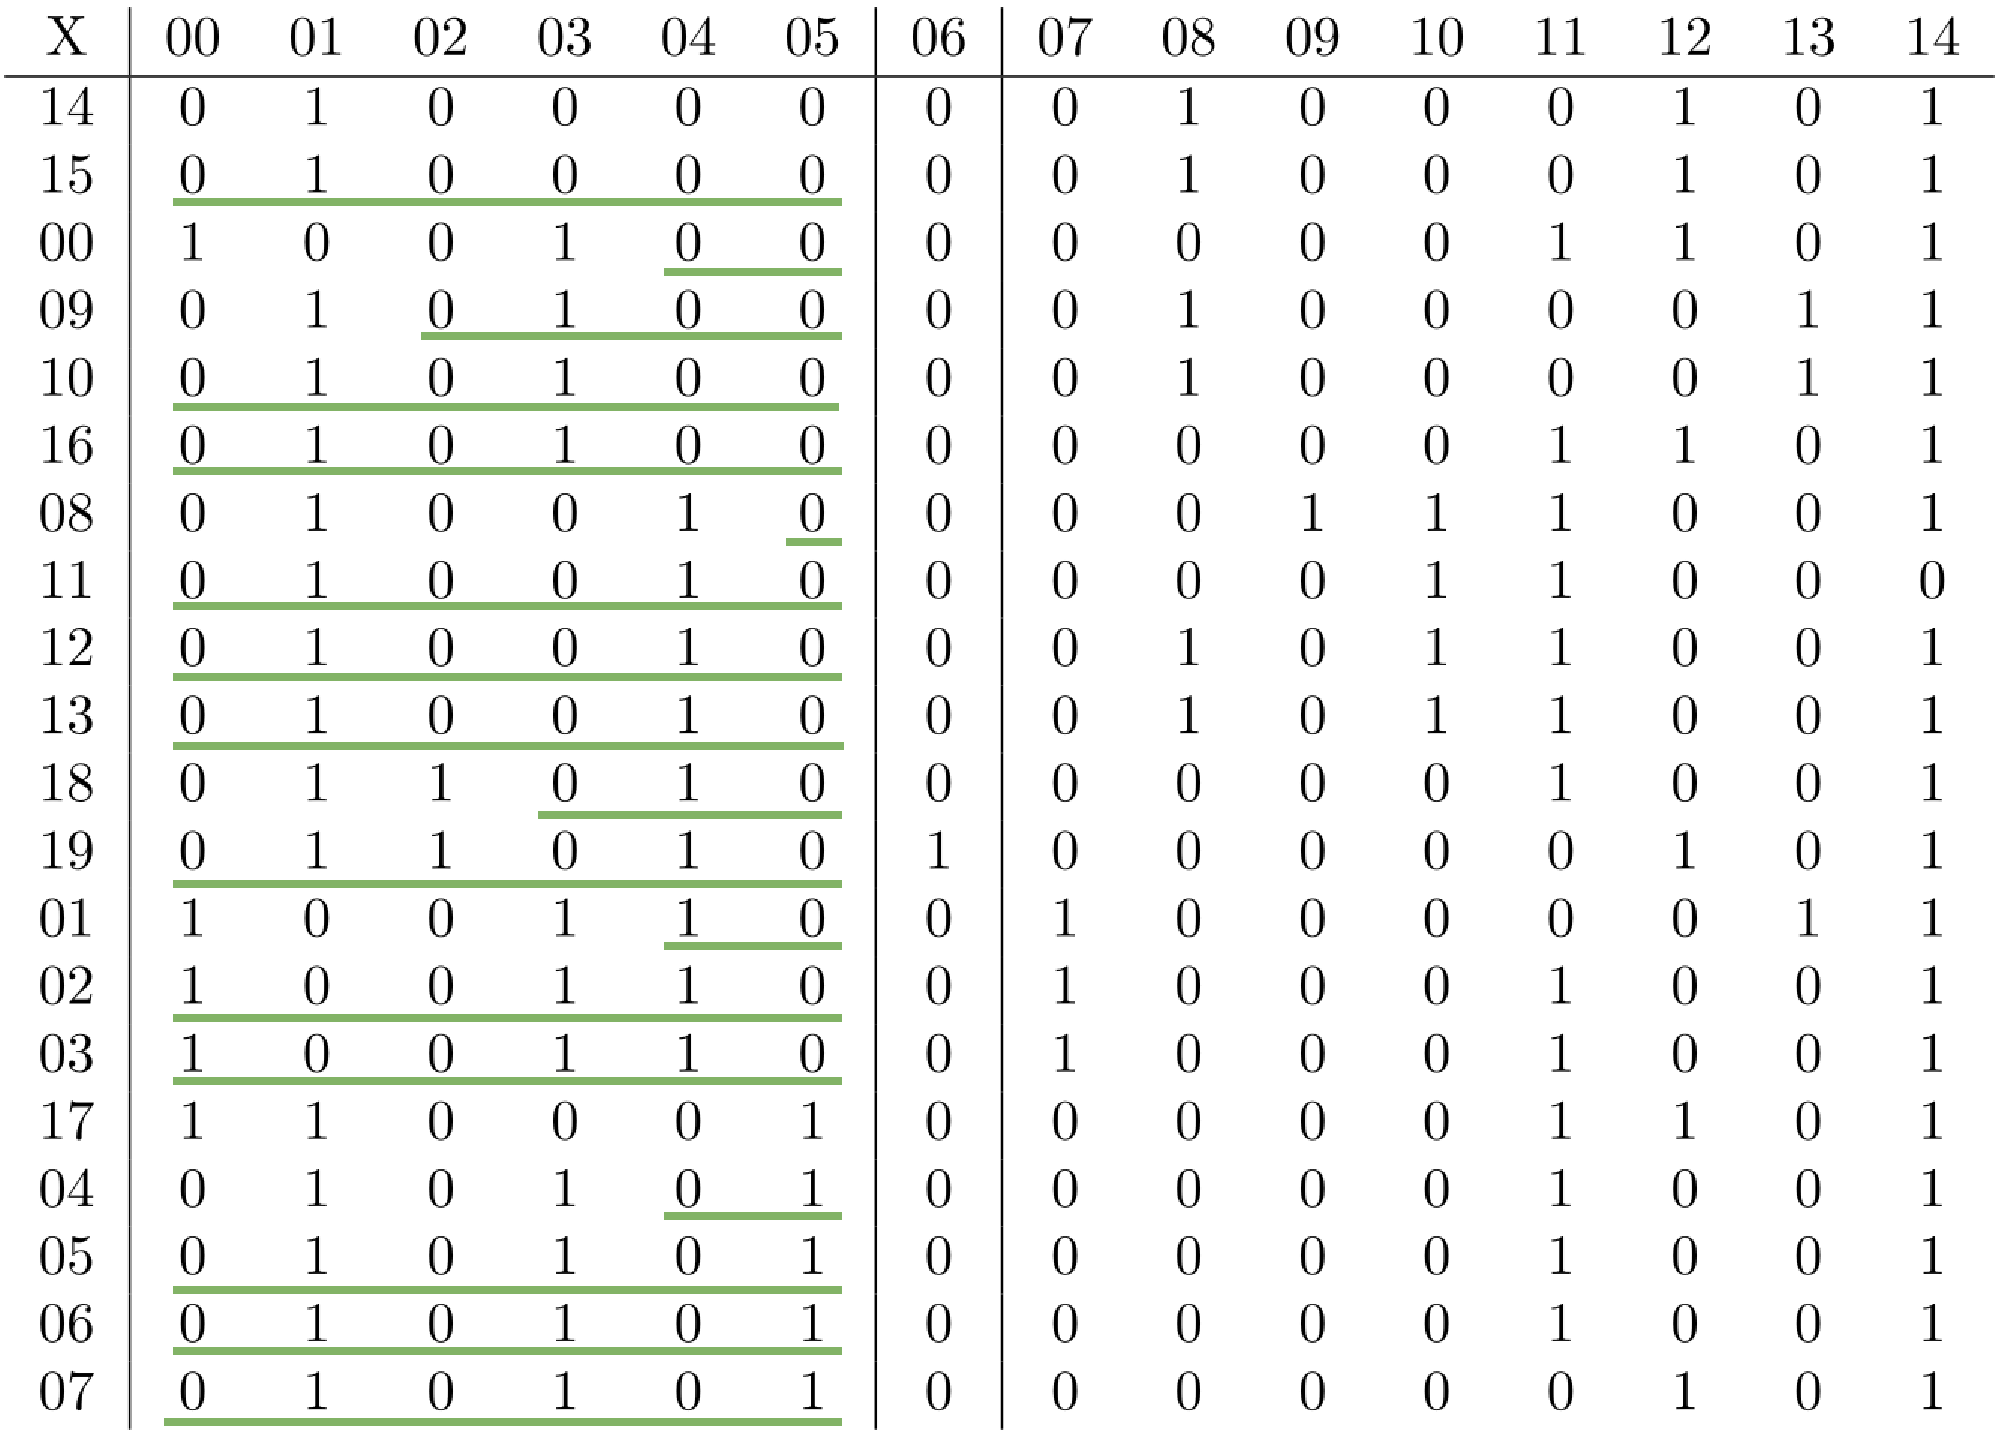
\includegraphics[scale = 0.325]{img/matrix1.pdf}
  \end{figure}
  \noindent
  Si ha, nel complesso:
  \[a_6=[14,15,0,9,10,16,8,11,12,13,18,19,1,2,3,17,4,5,6,7]\]
  \[\alpha_6=[2,12,13,14,16,17,18,19,6,3,4,7,8,9,0,1,5,15,10,11]\]
  \[d_6=[6,0,4,2,0,0,5,0,0,0,3,0,4,0,0,6,4,0,0,0]\]
  \[l_6=[0,6,2,4,6,6,1,6,6,6,3,6,2,6,6,0,2,6,6,6]\]
  Permutando $X$ con tutti gli $a_k$, si ottiene la seguente matrice $\PBWT$:
  \begin{table}[H]
  \centering
  \scriptsize
  \begin{tabular}{c|ccccccccccccccc}
    \tiny{$\PBWT$} & 00 & 01 & 02 & 03 & 04 & 05 & 06 & 07 & 08 & 09 & 10 & 11 & 12 & 13
    & 14 \\
    \hline
    00 & 1 & 1 & 0 & 1 & 1 & 0 & 0 & 0 & 1 & 0 & 0 & 1 & 1 & 1 & 1 \\
    01 & 1 & 1 & 0 & 1 & 1 & 0 & 0 & 0 & 1 & 0 & 0 & 1 & 1 & 1 & 1 \\
    02 & 1 & 1 & 0 & 1 & 1 & 1 & 0 & 0 & 0 & 1 & 1 & 1 & 0 & 1 & 1 \\
    03 & 1 & 1 & 0 & 1 & 1 & 0 & 0 & 0 & 1 & 0 & 0 & 1 & 1 & 0 & 1 \\
    04 & 0 & 1 & 0 & 1 & 0 & 1 & 0 & 0 & 1 & 0 & 0 & 1 & 1 & 0 & 1 \\
    05 & 0 & 1 & 0 & 1 & 0 & 1 & 0 & 0 & 0 & 0 & 0 & 1 & 0 & 0 & 1 \\
    06 & 0 & 1 & 0 & 1 & 0 & 1 & 0 & 0 & 0 & 0 & 0 & 1 & 0 & 0 & 0 \\
    07 & 0 & 1 & 0 & 1 & 1 & 1 & 0 & 0 & 0 & 0 & 0 & 0 & 1 & 0 & 1 \\
    08 & 0 & 1 & 0 & 0 & 1 & 0 & 0 & 0 & 1 & 0 & 0 & 0 & 1 & 0 & 1 \\
    09 & 0 & 1 & 0 & 1 & 0 & 0 & 0 & 0 & 1 & 0 & 0 & 0 & 0 & 0 & 1 \\
    10 & 0 & 1 & 0 & 1 & 1 & 0 & 0 & 0 & 0 & 0 & 0 & 1 & 1 & 0 & 1 \\
    11 & 0 & 1 & 0 & 0 & 1 & 0 & 1 & 1 & 0 & 0 & 0 & 1 & 0 & 0 & 1 \\
    12 & 0 & 1 & 0 & 0 & 1 & 0 & 0 & 1 & 0 & 0 & 0 & 0 & 0 & 0 & 1 \\
    13 & 0 & 1 & 0 & 0 & 0 & 0 & 0 & 1 & 0 & 0 & 0 & 0 & 0 & 0 & 1 \\
    14 & 0 & 1 & 0 & 0 & 0 & 0 & 0 & 0 & 0 & 0 & 0 & 0 & 0 & 0 & 1 \\
    15 & 0 & 0 & 0 & 0 & 0 & 0 & 0 & 0 & 0 & 0 & 0 & 0 & 0 & 0 & 1 \\
    16 & 0 & 0 & 0 & 1 & 0 & 0 & 0 & 0 & 0 & 0 & 0 & 1 & 0 & 0 & 1 \\
    17 & 1 & 0 & 1 & 0 & 0 & 0 & 0 & 0 & 0 & 0 & 1 & 1 & 0 & 0 & 1 \\
    18 & 0 & 0 & 1 & 0 & 0 & 0 & 0 & 0 & 0 & 0 & 1 & 1 & 0 & 0 & 1 \\ 
    19 & 0 & 1 & 0 & 0 & 0 & 0 & 0 & 0 & 0 & 0 & 1 & 1 & 0 & 0 & 1
  \end{tabular}
\end{table}
\end{esempio}
\subsection{Set-maximal exact match con aplotipo esterno}
Durbin, nel suo articolo, propone diversi algoritmi per l'uso effettivo della
sua trasformata. Ad esempio, viene proposto un algoritmo per il calcolo
di match interni a $X$ più lunghi di una lunghezza minima $L$ e uno per la
ricerca di tutti gli $\SMEM$ interni a $X$, in tempo lineare.\\
Di interesse per questa tesi è il cosiddetto \textbf{algoritmo 5}, usato
per computare tutti gli $\SMEM$ tra il panello $X$ e un
aplotipo esterno $z$, assumendo che $z$ abbia lo stesso numero di siti del
pannello. Quest'ultimo vincolo è dovuto al fatto 
che una colonna $k$ del
pannello e una posizione $k$ della query rappresentano il medesimo sito.\\ 
L'idea dietro l'algoritmo è quella di usare tre indici: $e_k$, $f_k$ e
$g_k$. Nel dettaglio $e_k$ tiene traccia dell'inizio del più lungo match,
terminante in colonna $k$, tra $z$ e un qualche $y_i^k$. Invece, l'intervallo
$[f_k,g_k)\subseteq[0,\ldots,M)$ identifica il sotto-intervallo di
$a_k$ contenente gli indici degli aplotipi che presentano tale match. Si noti
come viene ripresa l'idea, vista con la backward search per la
$\BWT$, di studiare un intervallo $[f_k,g_k)$ su $\SA_T$ per identificare i
match tra un pattern e un testo. In questo caso, però, tratta di una
``forward search''.
\begin{definizione}
  Dato un pannello $X$, con $M$ aplotipi/righe e $N$ siti/colonne, e un aplotipo
  query $z$, tale che $|z|=N$, si definisce uno $\SMEM$, iniziante in colonna
  $e_k$ e terminante il colonna 
  $k$, tra 
  la query $z$ e tutte le righe del pannello indicizzate dai valori compresi
  nell'intervallo $[f_k,g_k)$ in $a_k$, sse:
  \begin{equation}
    \label{eq:pbwtsmem}
    z[e_k,k)=y_i^k[e_k,k)\land z[e_k-1]\neq y_i^k[e_k-1], \forall\, i\mbox{
      t.c. }f_k\leq i < g_k
  \end{equation}
  Si noti che $g_k=M$ sse $y_{M-1}^k$ appartiene alle righe per le quali si ha
  tale $\SMEM$.
\end{definizione}
Bisogna capire come aggiornare $e_k$, $f_k$ e $g_k$ passando dalla
colonna $k$ alla colonna $k+1$. Per calcolare $[f_{k+1},g_{k+1})$, si procede
esattamente come visto per la 
backward search nella $\BWT$, selezionando il
sottointervallo non stretto di $[f_k,g_k)$ in cui si hanno aplotipi che possono
essere estesi 
a destra con il simbolo $z[k+1]$. L'idea è quella per cui, avendo
$f_{k+1}<g_{k+1}$, allora sicuramente si hanno ancora delle righe che presentano un
match che parte da $e_{k+1}=e_{k}$ e termina in $k$ che può essere esteso in
$k+1$. In caso contrario, avendo $f_{k+1}=g_{k+1}$, non si hanno match
estendibili e si può concludere che quelli terminanti in colonna $k$
erano effettivamente $\SMEM$. In questo secondo caso, bisogna aggiornare
$e_{k+1}$, 
ottenendo i relativi nuovi valori $f_{k+1}$ e $g_{k+1}$, al fine di trovare la
colonna da cui parte lo $\SMEM$ successivo e le righe del pannello per le quali
si ha tale $\SMEM$. \\
A questo punto, bisogna capire come funziona la
variante del backward-step introdotta per la $\BWT$, avendo che nella $\PBWT$ si
può parlare di forward-step/mapping. Tale funzione,
guidata dal carattere corrente dell'aplotipo query, permette di ottenere
$f_{k+1}$ e $g_{k+1}$ a partire da $f_k$ e $g_k$.\\ 
Per effettuare il mapping abbiamo bisogno di tre componenti, che
svolgono la medesima funzione di $\C$ e $\Occ$ per la
$\BWT$: 
\begin{enumerate}
  \item l'array $c$ tale per cui $c[k]=j$ sse la colonna $k$ contiene $j$
  occorrenze di valori pari a 0
  \item l'array $u_k$ tale per cui, alla colonna $k$-esima, $u_k[i]=j$ sse $j$ è
  il numero di occorrenze di valori pari a 0 prima dell'indice $i$ in $y^k[k]$ 
  \item l'array $v_k$ tale per cui, alla colonna $k$-esima, $v_k[i]=j$ sse $j$ è
  il numero di occorrenze di valori pari a 1 prima dell'indice $i$ in $y^k[k]$ 
\end{enumerate}
Tali valori possono essere computati e memorizzati in fase di costruzione della
$\PBWT$, come visibile direttamente nell'algoritmo \ref{algo:durbin1} per
quanto riguarda $u$ e $v$ (per l'array $c$ basterebbe tenere traccia del numero
di 0 incontrati nella colonna $k$-esima o sfruttare direttamente l'array $u$).\\
Sfruttando i valori di questi tre array possiamo quindi effettuare lo
step/mapping alla colonna successiva,
definito da una funzione:
\begin{equation}
  \label{eq:pbwtw1}
  w_k:\{0,\ldots,M\}\times\Sigma\to \{0,\ldots,M\}
\end{equation}
tale per cui:
\begin{equation}
  \label{eq:pbwtw2}
  w_k(i,\sigma)=
  \begin{cases}
    u_k[i]&\mbox{ se }\sigma=0\\
    v_k[i]+c[k]&\mbox{ se }\sigma=1
  \end{cases}
\end{equation}
Tale funzione è rappresentabile in pseudocodice come nell'algoritmo
\ref{algo:pbwtlf}. \\
Risulta interessante notare che:
\begin{equation}
  \label{eq:pbwt3}
  a_{k+1}\left[w_k\left(i,y_i^k[k]\right)\right]=a_k[i]
\end{equation}
Quindi, tale mapping permette di ``seguire'' una determinata riga
all'interno delle permutazioni dettate dai valori dei prefix array.
\begin{algorithm}
  \small
  \begin{algorithmic}[1]
    \Function{w}{$k,i,s, c_k, u_k, v_k$}
    \If{$s = 0$}
    \State \textbf{return} $u_k[i]$
    \Else
    \State \textbf{return} $c_k+v_k[i]$
    \EndIf
    \EndFunction
  \end{algorithmic}
  \caption{Algoritmo per il mapping nella PBWT.}
  \label{algo:pbwtlf}
\end{algorithm}
\begin{esempio}
  Si riprende l'esempio
  \ref{es:pbwt1}, ricordando che:
  \[a_5=[14,15,17,0,4,5,6,7,9,10,16,8,11,12,13,18,19,1,2,3]\]
  \[\alpha_5=[3,17,18,19,4,5,6,7,11,8,9,12,13,14,0,1,10,2,15,16]\]
  \[a_6=[14,15,0,9,10,16,8,11,12,13,18,19,1,2,3,17,4,5,6,7]\]
  \[\alpha_6=[2,12,13,14,16,17,18,19,6,3,4,7,8,9,0,1,5,15,10,11]\]
  Si ha, con $k=5$ e $i=2$, che:
  \[a_{6}\left[w_5\left(2,y_2^5[5]\right)\right]=a_5[2]\]
  Avendo:
  \[w_5\left(2,y_2^5[5]\right)=w_5\left(2,1\right)=v_5[2]+c[5]=0+15=15\]
  Avendo anche che:
  \[a_{6}[15]=17=a_5[2]\]
  Si conferma come con tale funzione si possa seguire la riga 17,
  capendo da quale riga della colonna permutata precedente arrivi.
\end{esempio}
\noindent
Pensando alla permutazione inversa del prefix array, si
ottiene un altro risultato interessante, che lega tale permutazione alla
funzione $w_k$:
% permettendo di ottenere risultati per la
% colonna $k+1$ a partire dalla colonna $k$-esima:
\begin{equation}
  \label{eq:pbwtw4}
  \alpha_{k+1}[i]=w_k(\alpha_k[i],x_i[k])
\end{equation}
\begin{esempio}
  Si riprendono i dati dell'esempio precedente e si calcola, sempre con
  $k=5$ e $i=2$:
  \[\alpha_{6}[2]=13=w_5(\alpha_5[2],x_2[5])=w_5(18,0)=13\]
  Come volevasi dimostrare.
\end{esempio}
L'ultima equazione ci suggerisce che la funzione $w_k$
consente il corretto aggiornamento di $f_k$ e $g_k$.
Definendo, infatti:
\begin{equation}
  \label{eq:pbwtq5}
  f_{k+1}=w_k(f_k,z[k])
\end{equation}
si ha che $f_{k+1}$ sarà l'indice, in $a_{k+1}$, della prima sequenza $y_j^k$,
con $j\geq f_k$, per la quale $y_j^k[k]=z[k]$. Analogamente, pensando alla prima
sequenza per cui si ha un mismatch dopo l'aggiornamento dell'intervallo, si
calcola: 
\begin{equation}
  \label{eq:pbwtq6}
  g_{k+1}=w_k(g_k,z[k])
\end{equation}
Si hanno, dopo il calcolo dei potenziali $f_{k+1}$ e $g_{k+1}$, due
possibili casi: 
\begin{enumerate}
  \item $f_{k+1}<g_{k+1}$. In questo caso ci sono ancora match,
  inizianti in $e_k$ e terminanti in $k$, che si estendono anche in $k+1$. In
  altri 
  termini, si 
  ha un sottointervallo non nullo di $[f_k, g_k)$ relativo a righe che 
  presentano $z[k+1]$ come simbolo in colonna $k+1$. In tal caso, si
  prosegue con l'iterazione, avendo $e_{k+1}=e_k$
  \item $f_{k+1}=g_{k+1}$. In questo caso non ci si sono match,
  inizianti in $e_k$ e terminanti in $k$, che sono anche estendibili in
  $k+1$. Bisogna, quindi, 
  annotare i match terminanti in $k-1$, ovvero gli $\SMEM$ con le righe
  indicizzate nell'intervallo
  $[f_k,g_k)$ su $a_k$, 
  e poi ricalcolare i nuovi $e_{k+1}$, $f_{k+1}$ e $g_{k+1}$. Il punto
  fondamentale per poter calcolare i nuovi indici è 
  che l'aplotipo $z$ si trova virtualmente o subito prima o
  subito dopo l'insieme di aplotipi indicizzati da $[f_k,g_k)$ su $a_k$, in
  colonna $k$ secondo il riordinamento inverso.
  Di conseguenza, si può inferire che, avendo $f_{k+1}=g_{k+1}$: 
  \begin{equation}
    \label{eq:pbwtsmem1}
    y_{f_{k+1}-1}^{k+1}\prec z\prec y_{f_{k+1}}^{k+1}
  \end{equation}
  Ne segue direttamente che:
  \begin{equation}
    \label{eq:pbwtsmem2}
    e_{k+1}\leq d_{k+1}[f_{k+1}]
  \end{equation}
  Il nuovo indice di partenza del match sarà almeno nella colonna
  indicata da $d_{k+1}[f_{k+1}]$, essendo esso calcolato tra $
  y_{f_{k+1}-1}^{k+1}$ e $ y_{f_{k+1}}^{k+1}$, fra le quali sequenze è
  virtualmente compresa la query $z$. \\
  Quindi, si considera come punto di partenza:
  \begin{equation}
    \label{eq:pbwtsmem3}
    e_{k+1}=d_{k+1}[f_{k+1}]-1
  \end{equation}
  Studiando $z[e_{k+1}]$, grazie al
  fatto che, per la nozione di divergence array e di ordinamento dei
  prefissi inversi con $0\prec 1$:
  \begin{equation}
    \label{eq:pbwtsmem4}
    y_{f_{k+1}-1}^{k+1}[e_{k+1}]=0\neq y_{f_{k+1}}^{k+1}[e_{k+1}]=1
  \end{equation}
  si hanno due casi possibili:
  \begin{enumerate}
    \item se tale valore è 0, allora, $z$ ha un match migliore
    con $y_{f_{k+1}-1}^{k+1}$ rispetto che con $y_{f_{k+1}}^{k+1}$. Si aggiorna,
    quindi, $e_{k+1}$, decrementandolo fino a che si ha match tra $z[e_{k+1}-1]$
    e $y_{f_{k+1}-1}^{k+1}[e_{k+1}-1]$. Infine, si decrementa $f_{k+1}$ fino a
    che $d_{k+1}[f_{k+1}]\leq e_{k+1}$, trovando quelle righe per le quali il
    divergence array non supera il valore di $e_{k+1}$. Si ottengono, in
    tal modo, le sequenze, nel riordinamento in $k+1$, che hanno un match da
    $e_{k+1}$ a $k+1$. Invece, $g_{k+1}$ resta fisso, avendo che
    $y_{g_{k+1}}^{k+1}$ presenta un
    mismatch in colonna $k+1$
    \item se tale valore è 1, allora, $z$ ha un match migliore
    con $y_{f_{k+1}}^{k+1}$ rispetto che con $y_{f_{k+1}-1}^{k+1}$. Si aggiorna,
    quindi, $e_{k+1}$, decrementandolo fino a che si ha match tra $z[e_{k+1}-1]$
    e $y_{f_{k+1}-1}^{k+1}[e_{k+1}-1]$. Infine, si incrementa $g_{k+1}$ fino a
    che $d_{k+1}[g_{k+1}]\leq e_{k+1}$, per lo stesso ragionamento del caso
    precedente. Si noti che è possibile ottenere $g_{k+1}=M$, avendo che tale
    valore risulta escluso in $[f_{k+1},g_{k+1})$. In tal modo si segnala che la
    riga indicizzata con $a_{k+1}[M-1]$, in colonna $k+1$, presenta un
    match. Invece, $f_{k+1}$ resta fisso, avendo che $y_{f_{k+1}}^{k+1}$ 
    presenta un mismatch in colonna $k+1$ 
  \end{enumerate}
\end{enumerate}
In termini di inizializzazione, per permettere il funzionamento dell'algoritmo,
si hanno: $f_0=g_0=e_0=0$.
% Quindi il primo step sarà già un caso in cui $f_k=g_k$ qualora $x_0[0]=y_0^0\neq
% z[0]$.
\begin{esempio}
  \label{es:algo5}
  Mostrare un esempio completo di esecuzione richiederebbe troppo spazio quindi
  ci si limita a mostrare cosa succede nel caso in cui, a un certo punto
  dell'esecuzione, $f_{k+1}=g_{k+1}$.\\
  Assumendo il pannello e la matrice $\PBWT$ visti all'esempio
  \ref{es:pbwt1}, con una query $z$, si identificano i
  seguenti $\SMEM$:
  \begin{figure}[H]
    \centering
    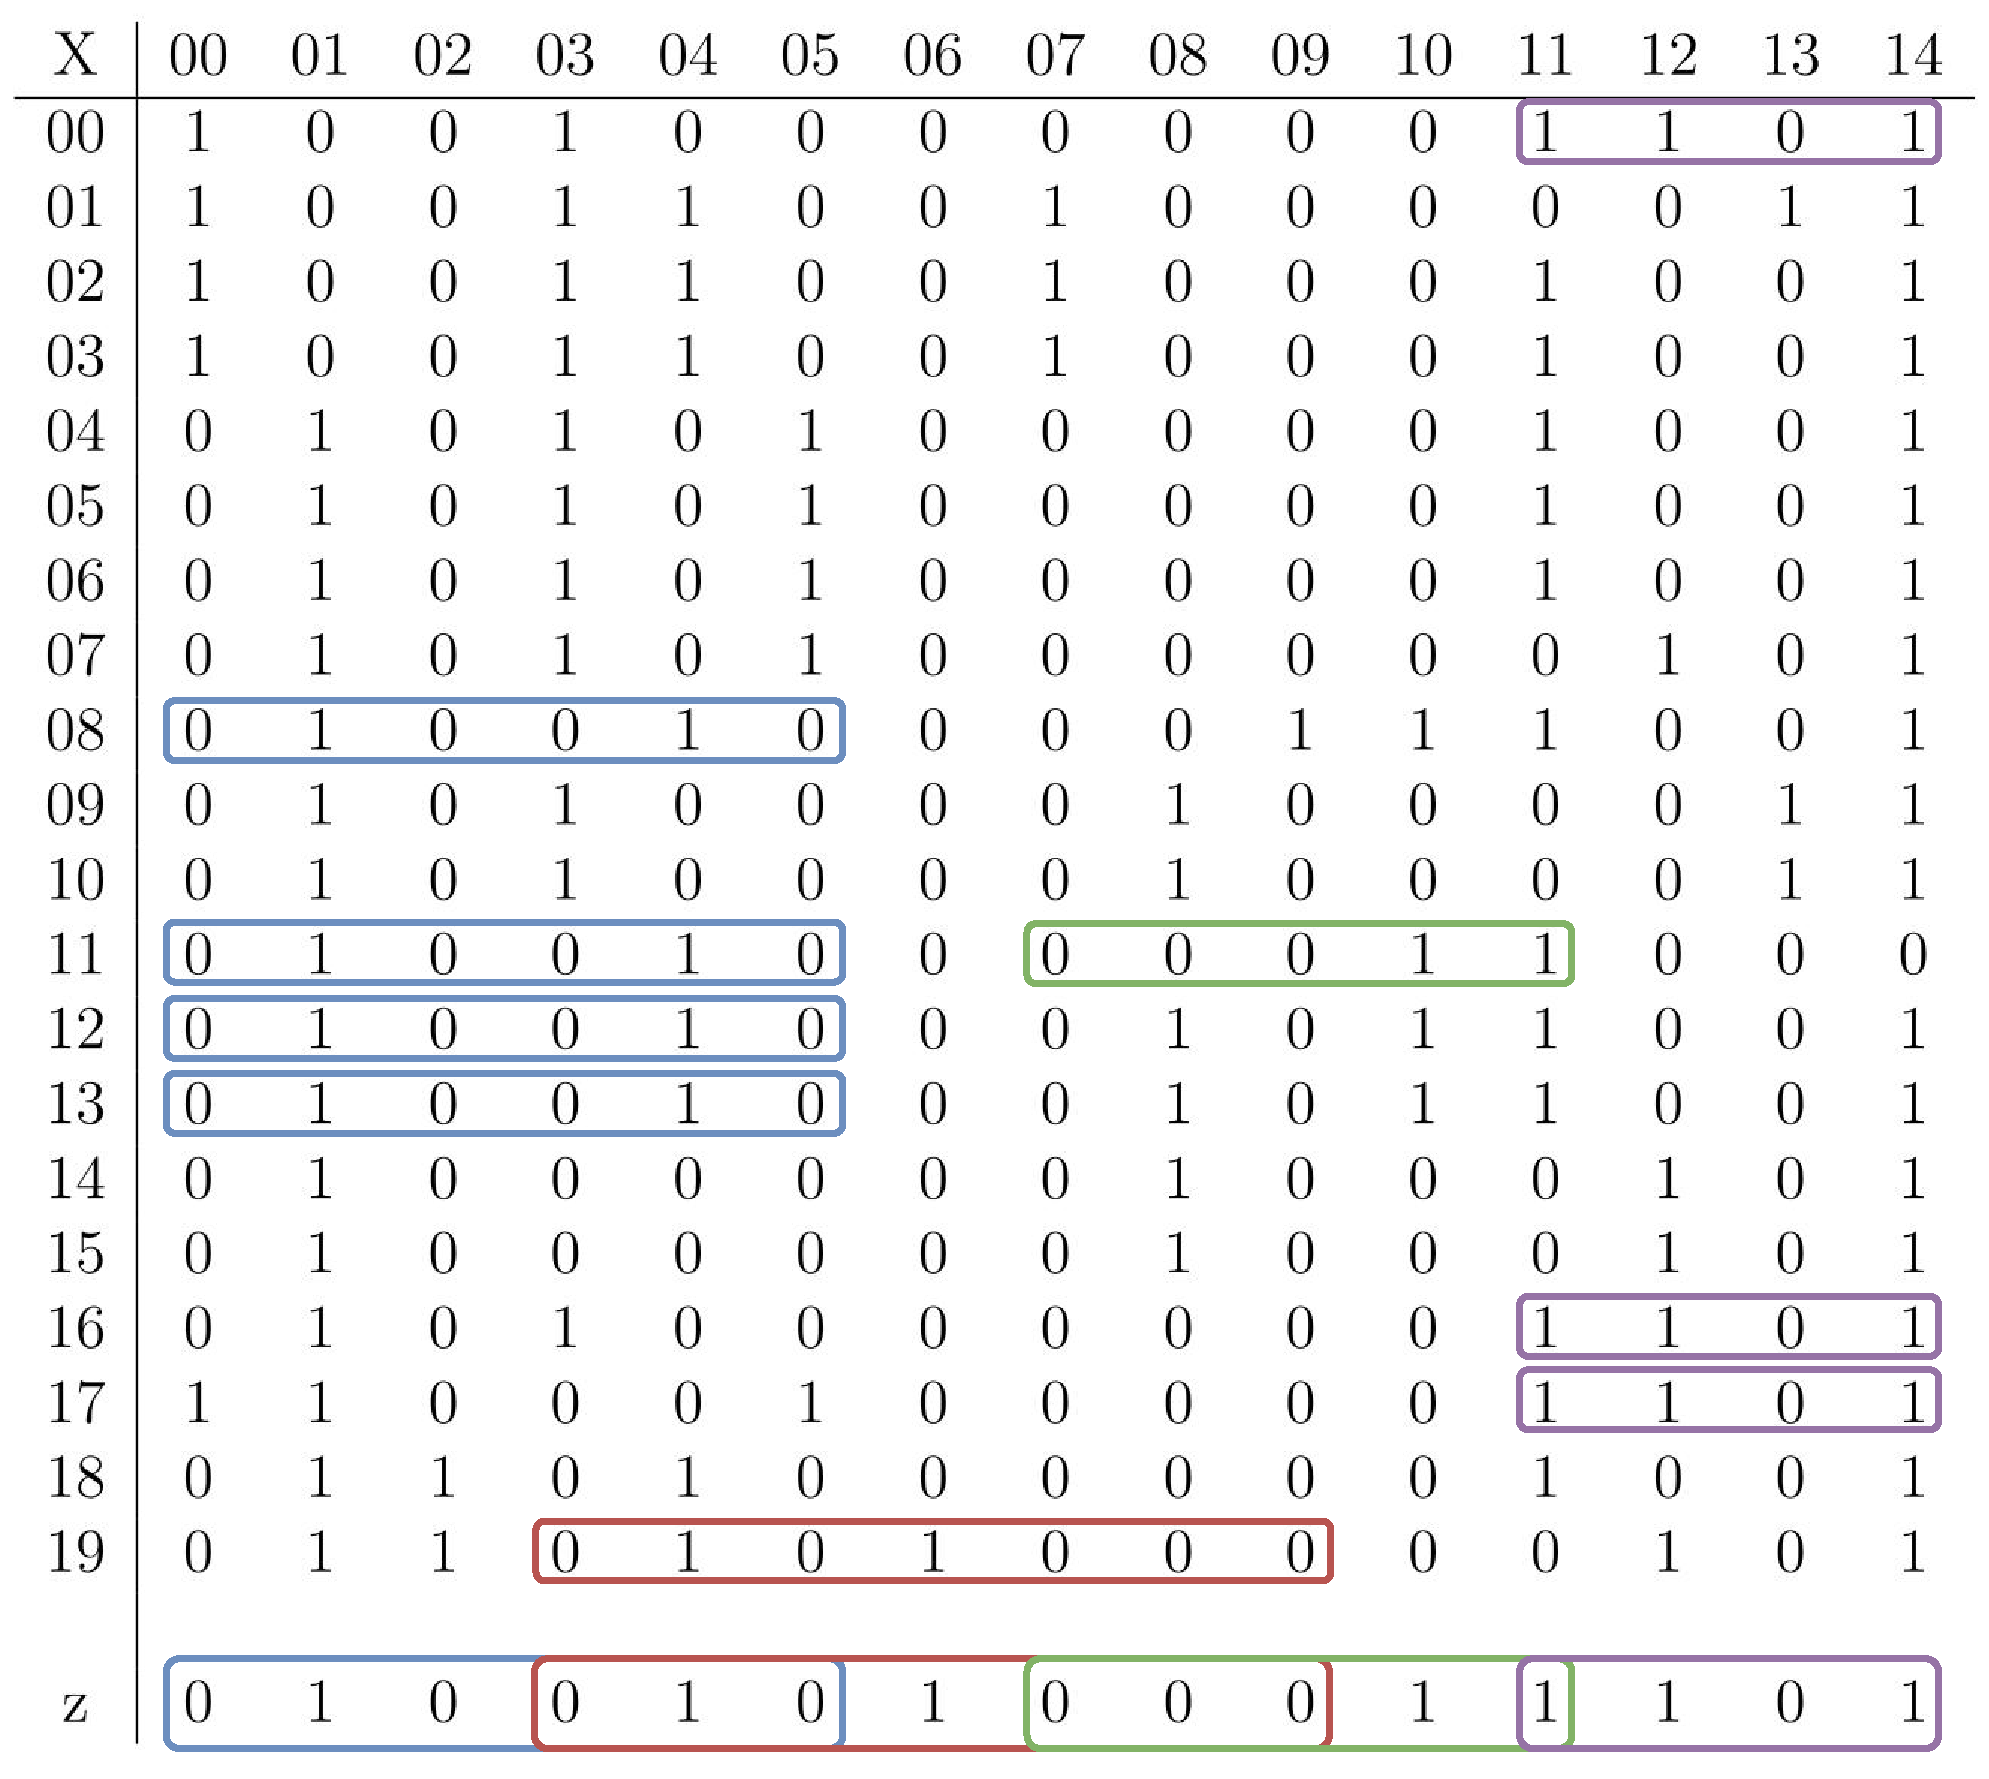
\includegraphics[scale = 0.365]{img/pbwtmatch.pdf}
  \end{figure}
  Assumendo di essere in colonna $k=6$ e avendo, dopo i calcoli fatti in colonna
  $k=5$, si ha che:
  \[f_6=6,\quad\quad g_6=10,\quad\quad e_6=0\]
  % \begin{itemize}
  %   \item $f_6=6$
  %   \item $g_6=10$
  %   \item $e_6=0$
  % \end{itemize}
  Tali valori segnalano che, a partire dalla colonne $0$ fino alla colonna
  $6-1=5$, si 
  hanno le righe nel range $[6,10)$ di $a_{6}$ che presentano un match con
  $z[0,5]$. Tali 
  righe sono, nel dettaglio, quelle indicizzate $\{8, 11, 12, 13\}$.\\
  Bisogna quindi computare $f_7$ e $g_7$. Assumendo che $z[6]=1$ e che:
  \[y^6=00000000000100000000,\,\,\,c[6]=19\]
  si calcolano:
  \[f_7=w_6(6,1)=v_6[6]+c[6]=0+19=19\]
  \[g_7=w_6(10,1)=v_6[10]+c[6]=0+19=19\]
  Avendo $f_7=g_7$ si procede, in primis, annotando gli $\SMEM$ terminanti in
  $k=5$.\\
  Seguendo l'algoritmo si ha un primo aggiornamento di $e_{k+1}$, che,
  avendo in memoria $d_7$, viene posto pari a: 
  \[e_7=d_7[19]-1=7-1=6\]
  Questo viene fatto in quanto l'aplotipo $z$ si trova o subito
  prima o subito dopo il blocco di aplotipi $[f_k,g_k)$.\\
  Essendo, inoltre, $z[e_7]=z[6]=1$, si procede aggiornando $g_7$ e tenendo fisso
  $f_7$, avendo $z[6]=1$. Si calcola $g_7$:
  \[g_7=f_7+1=20\]
  A questo punto, si segue la riga specificata da $f_7$ in $a_7$ a ritroso,
  partendo da $e_7-1$, fino a che si hanno match con $z$, aggiornando così il
  valore di $e_7$.\\
  In questo caso non si hanno altre operazioni, in quanto $g_7=M$ ma, qualora
  non lo fosse stato, si sarebbe incrementato $g_7$ fino a che il corrispondente
  $d_7[g_7]$ sarebbe stato minore o uguale di $e_7$, identificando tutte le
  nuove righe presentanti un match con $z[e_7, 6]$.
\end{esempio}
Secondo i
calcoli di Durbin, il suo algoritmo 5,
consultabile all'algoritmo 
\ref{algo:dur5}, ha complessità: 
\begin{equation}
  \label{eq:pbwtsmem5}
  \mathcal{O}(N+c)
\end{equation}
Tale risultato è così stimato in quanto si ritiene che il
numero di accessi ai cicli \texttt{while} interni sia limitato dalla costante
$c$, rappresentante il 
numero di $\SMEM$. Nonostante ciò, tale complessità temporale è ancora in
corso di studio in quanto si hanno in letteratura evidenze della sua non
correttezza. Un esempio è il paper di Naseri \cite{dpbwt}, dove si afferma che
l'intuizione per cui tale costante $c$ limiti superiormente gli accessi ai loop
innestati sia falsa. Si noti che nell'articolo non viene precisata una
nuova misura per la complessità dell'algoritmo ma solo che la stima di Durbin è
empiricamente accettabile come \textit{caso medio}:
\begin{equation}
  \label{eq:pbwtsmem6}
  Avg.\,\,\,\mathcal{O}(N+c)
\end{equation}
In ogni caso, una soluzione na\"{i}ve, impiegherebbe tempo:
\begin{equation}
  \label{eq:pbwtsmem7}
  \mathcal{O}(N^2M)
\end{equation}
Si comprende, quindi, come tale algoritmo e tale struttura siano stati
rivoluzionari per lo studio di pannelli di aplotipi.
\begin{algorithm}
  \begin{algorithmic}[1]   
    \Function{Find\_Set\_Maximal\_Matches\_With\_Z}{$z$}
    \State $e\gets 0,\,\,f\gets 0,\,\,f\gets 0$
    \For {$k\gets 0$ \textbf{to} $N$}
    \State $e,f,g\gets \mbox{\textit{Update\_Matches}}(k, z, e, f, g)$
    \EndFor
    \EndFunction
    \State
    \Function{Update\_Matches}{$k, z, e, f, g$}
    \State $f'\gets \W(k, f, z[k])$
    \State $g'\gets \W(k, g, z[k])$
    \If{$f'<g'$}
    \Comment\textit{{se $k$ è $N-1$ report degli $\SMEM$ da $e_k$ a $N-1$}}
    \State $e'\gets e_k$
    \Else
    \Comment{\textit{report degli $\SMEM$ da $e_k$ a $k$}}
    \State $e'\gets d_{k+1}[f']-1$
    \If{$z[e']=0$ \textbf{and} $f'>0$}
    \State $f'\gets g'-1$
    \State \textbf{while} $z[e'-1]=y_{f'}^{k+1}[e'-1]$ \textbf{do} $e'\gets
    e'-1$
    \State \textbf{while} $d_{k+1}[f']\leq e'$ \textbf{do} $f'\gets f'-1$
    \Else
    \State $g'\gets f'+1$
    \State \textbf{while} $z[e'-1]=y_{f'}^{k+1}[e'-1]$ \textbf{do}  $e'\gets
    e'-1$ 
    \State \textbf{while} $g'<M$ \textbf{and} $d_{k+1}[g']\leq e'$ \textbf{do}
    $g'\gets g'+1$ 
    \EndIf
    \EndIf
    \State \textbf{return} $e',f',g'$
    \EndFunction
  \end{algorithmic}
  \caption{\footnotesize{Algoritmo 5 di Durbin per il calcolo degli $\SMEM$ con
  aplotipo esterno.}}
  \label{algo:dur5}
\end{algorithm}
\subsubsection{Limiti spaziali}
Bisogna affrontare la tematica della complessità in spazio di tale
algoritmo. Si ipotizzi di non ricalcolare, colonna per colonna, tutti gli array  
necessari a costruire la $\PBWT$ e a permettere di computare la funzione
$w(i,\sigma)$, comportando
un'incremento dal punto di vista temporale per studiare più query
$z$.\\
Ricapitolando, per poter eseguire l'algoritmo 5, è necessario avere in
memoria con random access:
\begin{itemize}
  \item il pannello $X$, di dimensione $NM$
  \item l'insieme dei prefix array $a$, di dimensione $NM$
  \item l'insieme dei divergence array $d$, di dimensione $NM$
  \item gli array $u_k$ e $v_k$, per ogni colonna $k$, complessivamente
  di dimensione $2NM$ 
  \item l'array $c$, di dimensione $N$
\end{itemize}
Quindi, si ha una complessità in spazio pari a:
\begin{equation}
  \label{eq:pbwtsize}
  \mathcal{O}(NM)
\end{equation}
Nel dettaglio, Durbin stesso ha proposto una stima quantitativa della memoria
richiesta,
ovvero\footnote{\scriptsize{\url{https://github.com/richarddurbin/pbwt/blob/0de8d02df1b77146ded81e9e196991fdab520767/pbwtMatch.c\#L252}}}:
\begin{equation}
  \label{eq:pbwtsize2}
  13NM\mbox{ byte}
\end{equation}
Per poter capire meglio la problematica conseguente a tali richieste di spazio,
prendiamo, ad esempio, un pannello di 
dimensioni $N= 6.196.151$ e $M=4.908$. Ne segue che si necessitano 368GB di
memoria. Una stima 
sperimentale di tale richiesta di memoria può essere confermata con l'esecuzione
dell'implementazione ufficiale della
$\PBWT$\footnote{\url{https://github.com/richarddurbin/pbwt}}. Infatti,
monitorando  
con \texttt{time} il picco di memoria durante l'esecuzione, si ha che esso
corrisponde a 369GB. \\
L'alto uso di memoria richiesto dall'algoritmo 5 è 
stata la motivazione principale per cui si è sviluppata, in questa tesi
magistrale, una versione run-length encoded della $\PBWT$ che permettesse il
calcolo degli $\SMEM$ con un aplotipo esterno, in modo efficiente dal punto di
vista della memoria richiesta.
\subsection{Varianti della PBWT}
Negli anni immediatamente successivi all'articolo di Durbin, una miriade di
articoli e ricerche sono state svolte per migliorare la $\PBWT$, crearne
varianti o utilizzarla per portare a compimento vari studi. Non essendo tali
lavori direttamente correlati a questa tesi non 
verranno approfonditi ma, soprattutto nell'ottica delle prospettive futuri, è
bene citarne i principali.
\subsubsection{PBWT multiallelica}
La prima variante che si introduce è la \textbf{PBWT multiallelica} ($\MPBWT$),
proposta da Naseri et al. \cite{mpbwt} nel 2019. Questo 
lavoro estende la $\PBWT$ di Durbin, generalizzandola a un alfabeto
arbitrario. \\
Dal punto di vista delle motivazioni biologiche, questa soluzione risulta
fondamentale in quanto gli studi riportano come, nell'uomo, la presenza di
siti triallelici sia sotto stimata \cite{tri} \cite{tri2}, oltre che per lo
studio di specie multialleliche (soprattutto nel
mondo vegetale). \\
Dal punto di vista algoritmico, si sono generalizzati i concetti di
$c$, $u_k$ e $v_k$ visti nella $\PBWT$, ottenendo un vero e proprio
FM-index in grado di lavorare su alfabeto arbitrario $\Sigma$, con
conseguente forte aumento dello spazio richiesto in memoria. Invece, dal punto
di vista della complessità temporale, si ha che le stime asintotiche
degli 
algoritmi devono tenere conto della grandezza dell'alfabeto stesso, considerando
che questo fatto non
comporta particolari problematiche dal punto di vista dei tempi di
calcolo, essendo l'alfabeto di dimensioni ridotte. Infatti, le complessità
temporali della $\MPBWT$ sono moltiplicate
di un fattore $t=\left|\Sigma\right|$. Se tale valore è assunto
costante a inizio computazione, la
complessità temporale non subisce variazioni considerevoli poiché
difficilmente $t>>2$.
\subsubsection{PBWT con struttura LEAP}
Sempre nel 2019, Naseri et al. \cite{leap} hanno proposto una variante della
$\PBWT$ 
che permetta il calcolo di qualsiasi match, tra un aplotipo esterno e un
pannello, di lunghezza maggiore uguale a una 
lunghezza arbitraria $L$. Tale algoritmo è stato nominato
\textit{PBWT-query}. Inoltre, nello 
stesso articolo, hanno proposto
una struttura dati aggiuntiva, detta \textit{LEAP} (Linked
Equal/Alternating Position), che ottimizzava i tempi
dell'algoritmo per la PBWT-query, ottenendo l'algoritmo
\textit{L-PBWT-query}, al costo della 
memorizzazione di otto array aggiuntivi che permettono di effettuare dei
salti nella matrice $\PBWT$ (salvando gli indici del precedente/prossimo
valore nella colonna uguale/diverso) e di memorizzare gli indici dei valori
nel divergence array relativi a tali indici.
Da un punto di vista computazionale, si noti che la complessità in tempo
dell'algoritmo 
per la PBWT query, con match di lunghezza minima $L$, è:
\begin{equation}
  \label{eq:leap1}
  \mathcal{O}(N+c(R-L+1))
\end{equation}
con:
\begin{itemize}
  \item $R$ lunghezza media dei match
  \item $c$ numero totale dei match
\end{itemize}
In merito alla complessità in tempo dell'algoritmo L-PBWT-query si ha che, al
costo di $8NM$ interi aggiuntivi in memoria, con $N$ e $M$ dimensioni del
pannello, essa è proporzionale a: 
\begin{equation}
  \label{eq:leap2}
  \mathcal{O}(N+c)
\end{equation}
\subsubsection{PBWT dinamica}
Sanaullah et al. \cite{dpbwt}, nel 2021, hanno proposto la \textbf{Dynamic PBWT}
($\DPBWT$), 
al fine di superare le limitazioni imposte dalle strutture
statiche usate nella $\PBWT$ di Durbin. Si è quindi pensato di sostituire
l'uso degli array con l'uso di linked list, ovvero strutture dati
dinamiche.
Questo ha portato all'aggiornamento
efficiente della matrice $\PBWT$, all'aggiunta di un nuovo aplotipo nel
pannello o alla rimozione di uno già presente.\\
Dal punto di vista computazionale, è interessante notare come le
implementazioni degli algoritmi di Durbin presentano la medesima complessità
asintotica di quelli basati sull'uso di tali strutture dinamiche. Ad
esempio, la creazione della $\DPBWT$ richiede tempo:
\begin{equation}
  \label{eq:dpbwt}
  \mathcal{O}(NM)
\end{equation}
Invece, l'aggiunta e la rimozione di un aplotipo sono entrambe in tempo:
\begin{equation}
  \label{eq:dpbwt1}
  Avg.\,\,\,\mathcal{O}(N)
\end{equation}
\subsubsection{PBWT con wildcard}
La tematica dei dati mancanti è una tematica aperta in
bioinformatica. I sequenziatori presentano un range d'errore
dall'1\% al 15\%, si ha a volte un basso coverage (ovvero il numero di
read che contengono la base sequenziata per un certo locus del genoma) e la fase
di assemblaggio del genoma può comportare errori. Questo, in fase di produzione
dei pannelli, implica che possa accadere che non si sappia quale sia l'allele
corretto per un individuo, riferendosi a un certo sito. \\
Nel 2020, Williams e Mumey \cite{williams} hanno proposto l'uso della
$\PBWT$ \textbf{con 
  wildcard} al fine di disegnare un algoritmo in grado di calcolare determinati
match interni a un pannello biallelico con dati mancanti, rappresentati come
wildcard mediante il simbolo ``*'' (avendo quindi, come alfabeto,
$\Sigma=\{0,1,*\}$).\\ 
In termini computazionali, gli autori sono riusciti a formulare un algoritmo in
grado di calcolare questi $T$ match interni al pannello in tempo: 
\begin{equation}
  \label{eq:pbwtwild}
  \mathcal{O}(NMT)
\end{equation}
\subsubsection{IMPUTE5}
Per citare un uso della $\PBWT$, si può introdurre il concetto di
\textit{genotype 
  imputation}, ovvero il processo con il quale si predicono genotipi non ancora
osservati in un campione di individui, usando un pannello di aplotipi. Questo
tipo di studio si basa sui dati prodotti dai \textbf{GWAS} (Genome-wide
    association studies), studi il cui scopo è quello di esaminare multipli
genomi alla ricerca di associazioni tra varianti genetiche e malattie (o
outcome specifici delle stesse), identificando varianti genomiche che sono
statisticamente associate al rischio di una malattia.\\ 
A tal fine, nel 2020, Rubinacci et al. \cite{impute5} hanno proposto
\textbf{IMPUTE5}, un metodo basato sulla $\PBWT$ per la genotype 
  imputation, in grado di studiare, in ottica GWAS, pannelli di grandi
  dimensioni. 
\subsection{Una prima proposta run-length encoded}
\label{subsectravis}
A fine 2021, Gagie et al. \cite{tricks} hanno iniziato a teorizzare una variante
run-length encoded della $\PBWT$, cercando di basarsi sui risultati
già ottenuti sulla $\BWT$ con la $\RLBWT$.
Pensando alla costruzione della $\PBWT$, con $M$ individui e $N$ siti, si
ha che ogni colonna della 
matrice $\PBWT$ è ottenuta tramite la permutazione data dal prefix
  array. Denotiamo tale permutazione, alla colonna $k$, con $\pi_k$, $\forall\,
0\leq k<N$. 
Ipotizziamo di voler studiare la riga $i$-esima del pannello originale. Si
ha che, al variare della colonna $k$ sulla matrice $\PBWT$, la posizione
della riga $i$ è ricostruibile applicando le varie permutazioni:
\begin{equation}
  \label{eq:pbwttrick}
  i, \pi_0(i), \pi_1(\pi_0(i)),\ldots,
  \pi_{N-1}(\cdots(\pi_1(\pi_0(i)))\cdots)
\end{equation}
Il punto fondamentale, relativo al run-length encoding, si ritrova nel fatto che
l'autore asserisce: 
\begin{center}
  \textit{Notice $\pi_k$ can be stored in space proportional to the number of
    runs in the $k$th column of the $\PBWT\,\ldots$} 
\end{center}
Nell'articolo si propone una struttura dati formata da $N$ ``tabelle''
dove la $j$-esima riga della $k$ tabella contiene: 
\begin{itemize}
  \item l'indice $p$ di inizio della $j$-esima run nella colonna $k$ della
   matrice $\PBWT$
  \item il valore $\pi_k(p)$, avendo che:
  \begin{equation}
    \label{eq:pbwttrick1}
    \pi_k(p)=
    \begin{cases}
      p-v_k[p]&\mbox{if } y_p^k[k]=0\\
      c[k]+v_k[p]-1&\mbox{if } y_p^k[k]=1\\
    \end{cases}
  \end{equation}
  \item l'indice della run contenente il simbolo $\pi_k(p)$ nella colonna $k+1$
  della matrice $\PBWT$
  \item un booleano che specifica se la prima run è composta da simboli
  $\sigma=0$. Si noti che tale valore non è esplicitato nell'articolo, ma
  risulta necessario per ottenere il simbolo corrispondente a una qualsiasi run
\end{itemize}
Il paper presenta anche il metodo per l'estrazione della $i$-esima
riga. Inizialmente, si cerca la riga relativa alla run nella prima
``tabella'', 
con indice di testa $p$, contenente l'indice $i$. Si noti che tale
``tabella'', relativa alla colonna $k=0$, non presenta permutazioni e quindi  
l'indice $i$ del pannello è anche l'indice $i$ della matrice $\PBWT$.
Si può calcolare, quindi, la permutazione per l'indice $i$ (alla prima
operazione si avrà $k=0$):
\begin{equation}
  \label{eq:pbwttrick2}
  \pi_k(i)=\pi_k(p)+i-p
\end{equation}
Si identifica, poi, la riga relativa alla run contenente il simbolo $\pi_k(p)$
nella ``tabella'' successiva e si scansionano le righe di tale tabella, a
partire da quella appena identificata, fino a trovare la run che contiene
$\pi_k(i)$ (alla prima
operazione si avrà $k=0$). Infine, si estrae il simbolo relativo a tale run.
Ripetendo la procedura per ogni colonna $k$, a partire dal computo della
permutazione, si 
può calcolare la riga $i$-esima del pannello.\\
Inoltre,
vengono proposte ulteriori ottimizzazioni, basate sul metodo detto
\textit{fractional cascading}. Con tale rappresentazione, si riesce a ridurre il
numero di run che devono essere scansionate, al costo di una
maggior richiesta di spazio. Infatti, aumentando il numero totale di
righe in tutte le tabelle di un fattore al più $\left(1+\frac{1}{d}\right)$, è
possibile garantire che si avranno al più $d$ iterazioni, in ogni tabella, per
ottenere l'estrazione del simbolo desiderato.
Per ulteriori dettagli si rimanda al paper di riferimento \cite{tricks}.
\begin{esempio}
   Supponendo di voler ricostruire la riga $i=9$ e assumendo la seguente matrice
   $\PBWT$, con in rosso i simboli appartenenti alla riga 9: 
   \begin{table}[H]
     \centering
     \scriptsize
     \begin{tabular}{c|ccccccccccccccc}
       X & 00 & 01 & 02 & 03 & 04 & 05 & 06 & 07 & 08 & 09 & 10 & 11 \\
       \hline
       00 & 1 & 1 & 0 & 0 & 0 & 1 & 0 & 0 & 1 & 1 & 1 & 1 \\
       01 & 1 & 1 & 0 & 0 & 0 & 1 & 0 & 0 & 1 & 1 & {\color{nordred}\textbf{\underline{1}}}
                                                                & 1 \\
       02 & 1 & 1 & 1 & 0 & 0 & 0 & 1 & 1 & 1 & 0 & 1 & 1 \\
       03 & 1 & 1 & 0 & {\color{nordred}\textbf{\underline{0}}} & {\color{nordred}\textbf{\underline{0}}}
                                  & {\color{nordred}\textbf{\underline{1}}} & 0 & 0 & 1 & 1
                                                           & 0 & 1 \\
       04 & 1 & 0 & 1 & 0 & 0 & 1 & 0 & 0 & 1 & 1 & 0 & 1 \\
       05 & 1 & 0 & 1 & 0 & 0 & 0 & 0 & 0 & 1 & {\color{nordred}\textbf{\underline{0}}} & 0
                                                                & 1 \\
       06 & 1 & 0 & 1 & 0 & 0 & 0 & 0 & 0 & 1 & 0 & 0 & 0 \\
       07 & 1 & 1 & 1 & 0 & 0 & 0 & 0 & 0 & 0 & 1 & 0 & 1 \\
       08 & 0 & 1 & {\color{nordred}\textbf{\underline{0}}} & 0 & 0 & 1 & 0 & 0 & 0 & 1 & 0
                                                                & 1 \\
       09 & {\color{nordred}\textbf{\underline{1}}} & 0 & 0 & 0 & 0 & 1 & 0 & 0 & 0 & 0 & 0
                                                                & 1 \\
       10 & 1 & 1 & 0 & 0 & 0 & 0 & 0 & 0 & 1 & 1 & 0 & 1 \\
       11 & 0 & 1 & 0 & 1 & 1 & 0 & 0 & 0 & 1 & 0 & 0 & 1 \\
       12 & 0 & 1 & 0 & 0 & 1 & 0 & 0 & 0 & 0 & 0 & 0 & 1 \\
       13 & 0 & 0 & 0 & 0 & 1 & 0 & 0 & 0 & 0 & 0 & 0 & 1 \\
       14 & 0 & 0 & 0 & 0 & 0 & 0 & 0 & 0 & {\color{nordred}\textbf{\underline{0}}} & 0 & 0
                                                                & 1 \\
       15 & 0 & 0 & 0 & 0 & 0 & 0 & 0 & {\color{nordred}\textbf{\underline{0}}} & 0 & 0 & 0
                                                                & 1 \\
       16 & 1 & 0 & 0 & 0 & 0 & 0 & {\color{nordred}\textbf{\underline{0}}} & 0 & 1 & 0 & 0
                                                                & 1 \\
       17 & 0 & {\color{nordred}\textbf{\underline{0}}} & 0 & 0 & 0 & 0 & 0 & 1 & 1 & 0 & 0
                                                                & 1 \\
       18 & 0 & 0 & 0 & 0 & 0 & 0 & 0 & 1 & 1 & 0 & 0
                                                                & {\color{nordred}\textbf{\underline{1}}} \\ 
       19 & 0 & 0 & 0 & 0 & 0 & 0 & 0 & 1 & 1 & 0 & 0 & 1 \\
     \end{tabular}
   \end{table}
   \newpage
   \noindent
   si costruiscono le seguenti tabelle \cite{tricks}:
   \begin{figure}[H]
     \centering
     \footnotesize
     %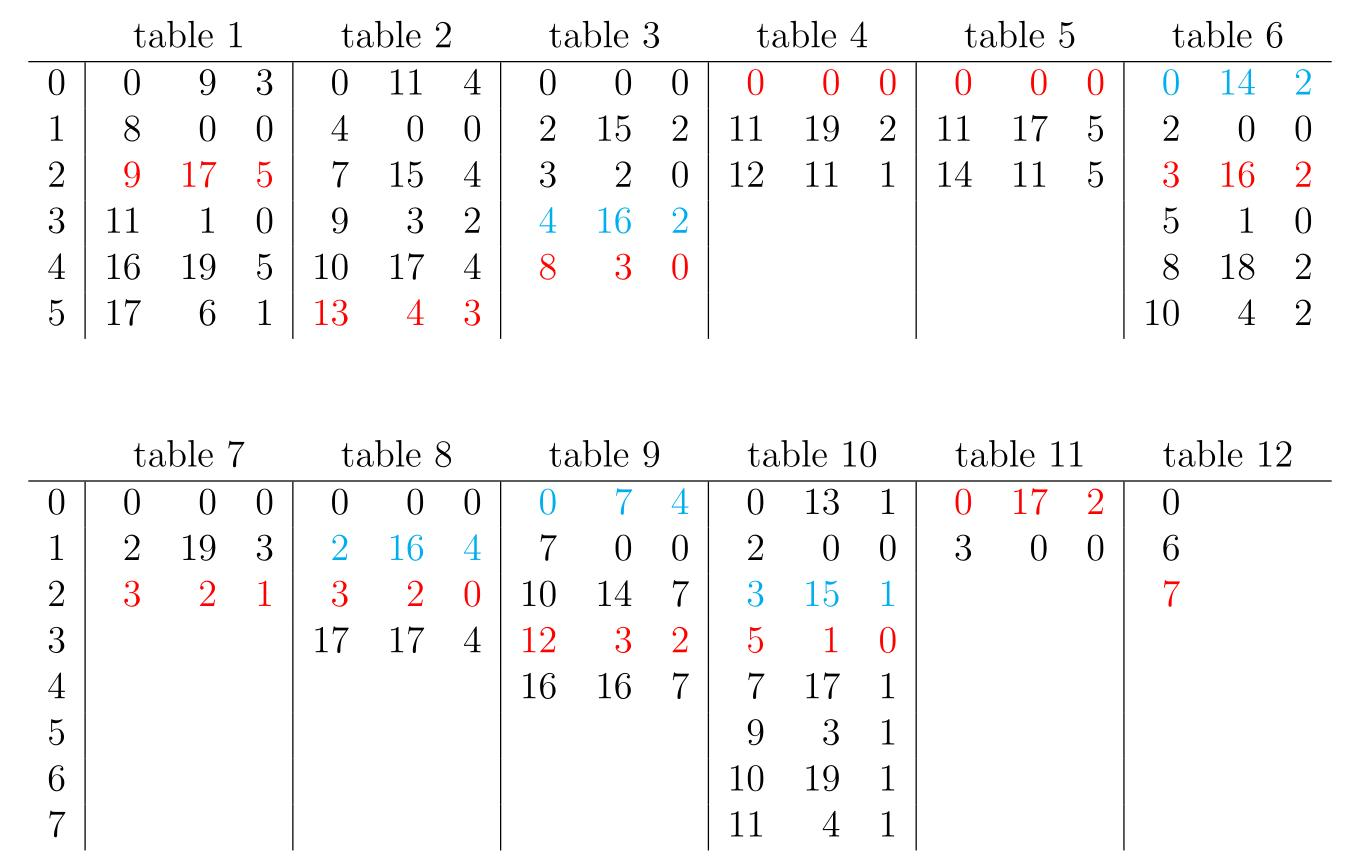
\includegraphics[scale=0.3]{img/trick.jpg}
     %\resizebox{0.75\textwidth}{!}
     {\begin{tabular}{r|rrr|rrr|rrr|rrr|rrr|rrr}
        \multicolumn{1}{c}{} &
                               \multicolumn{3}{c}{table 00} &
                                                             \multicolumn{3}{c}{table 01} &
                                                                                           \multicolumn{3}{c}{table 02} &
                                                                                                                         \multicolumn{3}{c}{table 03} &
                                                                                                                                                       \multicolumn{3}{c}{table 04} &
                                                                                                                                                                                     \multicolumn{3}{c}{table 05} \\
        \hline
        0 &  0 &  9 &  3 &  0 & 11 &  4 &  0 &  0 &  0 &  \textcolor{nordred}{0} &  \textcolor{nordred}{0} &  \textcolor{nordred}{0}
                                        &  \textcolor{nordred}{0} &  \textcolor{nordred}{0} &  \textcolor{nordred}{0}
                                                       &  \textcolor{nordcyan}{0} & \textcolor{nordcyan}{14} &  \textcolor{nordcyan}{2} \\
        1 &  8 &  0 &  0 &  4 &  0 &  0 &  2 & 15 &  2 & 11 & 19 &  2 & 11 & 17 &  5 &  2 &  0 &  0 \\
        2 &  \textcolor{nordred}{9} & \textcolor{nordred}{17} &  \textcolor{nordred}{5}
                                                                                                                       &  7 & 15 &  4 &  3 &  2 &  0 & 12 & 11 &  1 & 14 & 11 &  5 &  \textcolor{nordred}{3} & \textcolor{nordred}{16} &  \textcolor{nordred}{2} \\
        3 & 11 &  1 &  0 &  9 &  3 &  2 &  \textcolor{nordcyan}{4} & \textcolor{nordcyan}{16} &  \textcolor{nordcyan}{2}
                         &    &    &    &    &    &    &  5 &  1 &  0 \\
        4 & 16 & 19 &  5 & 10 & 17 &  4 &  \textcolor{nordred}{8} &  \textcolor{nordred}{3} &  \textcolor{nordred}{0}
                         &    &    &    &    &    &    &  8 & 18 &  2 \\
        5 & 17 &  6 &  1 & \textcolor{nordred}{13} &  \textcolor{nordred}{4} &  \textcolor{nordred}{3}
          &    &    &    &    &    &    &    &    &    & 10 &  4 &  2 \\
        \multicolumn{7}{c}{} \\[3ex]
        \multicolumn{1}{c}{} &
                               \multicolumn{3}{c}{table 06} &
                                                             \multicolumn{3}{c}{table 07} &
                                                                                           \multicolumn{3}{c}{table 08} &
                                                                                                                         \multicolumn{3}{c}{table 09} &
                                                                                                                                                        \multicolumn{3}{c}{table 10} &
                                                                                                                                                                                       \multicolumn{3}{c}{table 11} \\
        \hline
        0 &  0 &  0 &  0 &  0 &  0 &  0 &  \textcolor{nordcyan}{0} &  \textcolor{nordcyan}{7} &  \textcolor{nordcyan}{4}
                         &  0 & 13 &  1 &  \textcolor{nordred}{0} & \textcolor{nordred}{17} &  \textcolor{nordred}{2}
                                                       &  0 & \\
        1 &  2 & 19 &  3 &  \textcolor{nordcyan}{2} & \textcolor{nordcyan}{16} &  \textcolor{nordcyan}{4}
          &  7 &  0 &  0 &  2 &  0 &  0 &  3 &  0 &  0 &  6 & \\
        2 &  \textcolor{nordred}{3} &  \textcolor{nordred}{2} &  \textcolor{nordred}{1}
                                                                                                                       &  \textcolor{nordred}{3} &  \textcolor{nordred}{2} &  \textcolor{nordred}{0}
          & 10 & 14 &  7 &  \textcolor{nordcyan}{3} & \textcolor{nordcyan}{15} &  \textcolor{nordcyan}{1}
                                        &    &    &    &  \textcolor{nordred}{7} & \\
        3 &    &    &    & 17 & 17 &  4 & \textcolor{nordred}{12} &  \textcolor{nordred}{3} &  \textcolor{nordred}{2}
                         &  \textcolor{nordred}{5} &  \textcolor{nordred}{1} &  \textcolor{nordred}{0} &    &    &    &    & \\
        4 &    &    &    &    &    &    & 16 & 16 &  7 &  7 & 17 &  1 &    &    &    &    & \\
        5 &    &    &    &    &    &    &    &    &    &  9 &  3 &  1 &    &    &    &    & \\
        6 &    &    &    &    &    &    &    &    &    & 10 & 19 &  1 &    &    &    &    & \\
        7 &    &    &    &    &    &    &    &    &    & 11 &  4 &  1 &    &    &    &    &
      \end{tabular}
    }

  \end{figure}
  Nelle tabelle, in rosso, si hanno le varie $\pi_k(i)$,
  ottenute, 
  se necessario, iterando a partire dalle $\pi_k(p)$, segnalate in azzurro. \\
  Numericamente si hanno i seguenti calcoli, ovvero i diversi
  $\pi_j(i)=\pi_j(p)+i-p$
  relativi alle permutazioni in colonna $k$, per l'estrazione della riga $9$:
  \begin{multicols}{2}
    \begin{itemize}
      \item $\pi_{0}(9)=17+9-9=17$
      \item $\pi_{1}(17)=4+17-13=8$
      \item $\pi_{2}(8)=4+8-8=3$
      \item $\pi_{3}(3)=0+3-0=3$
      \item $\pi_{4}(3)=0+3-0=3$
      \item $\pi_{5}(3)=16+3-3=16$
      \item $\pi_{6}(16)=2+16-3=15$
      \item $\pi_{7}(15)=2+15-3=14$
      \item $\pi_{8}(14)=3+14-12=5$
      \item $\pi_{9}(5)=1+5-5=1$
      \item $\pi_{10}(1)=17+1-0=18$
      % \item $\pi_{12}(3)=16+3-3=16$        
    \end{itemize}
  \end{multicols}
  Sfruttando il valore booleano (non rappresentato nelle tabelle) che indica con
  che simbolo inizia una colonna 
  della matrice $\PBWT$ e
  sapendo che si alternano run con simboli $\sigma=0$ e
  $\sigma=1$ (pannello binario), si può ricostruire la riga 9 del pannello
  originale: 
  $x_9=100001000011$.
\end{esempio}
Si segnala che, nel paper, non vengono specificati metodi per
effettuare query a 
questa struttura dati, ma viene solo indicata la possibilità di interrogare
tale struttura a tabelle.
% LocalWords:  pseudocodice aplotipi mismatch
